\documentclass[11pt,preprint, authoryear]{elsarticle}

\usepackage{lmodern}
%%%% My spacing
\usepackage{setspace}
\setstretch{1.2}
\DeclareMathSizes{12}{14}{10}{10}

% Wrap around which gives all figures included the [H] command, or places it "here". This can be tedious to code in Rmarkdown.
\usepackage{float}
\let\origfigure\figure
\let\endorigfigure\endfigure
\renewenvironment{figure}[1][2] {
    \expandafter\origfigure\expandafter[H]
} {
    \endorigfigure
}

\let\origtable\table
\let\endorigtable\endtable
\renewenvironment{table}[1][2] {
    \expandafter\origtable\expandafter[H]
} {
    \endorigtable
}


\usepackage{ifxetex,ifluatex}
\usepackage{fixltx2e} % provides \textsubscript
\ifnum 0\ifxetex 1\fi\ifluatex 1\fi=0 % if pdftex
  \usepackage[T1]{fontenc}
  \usepackage[utf8]{inputenc}
\else % if luatex or xelatex
  \ifxetex
    \usepackage{mathspec}
    \usepackage{xltxtra,xunicode}
  \else
    \usepackage{fontspec}
  \fi
  \defaultfontfeatures{Mapping=tex-text,Scale=MatchLowercase}
  \newcommand{\euro}{€}
\fi

\usepackage{amssymb, amsmath, amsthm, amsfonts}

\def\bibsection{\section*{References}} %%% Make "References" appear before bibliography


\usepackage[round]{natbib}

\usepackage{longtable}
\usepackage[margin=2.3cm,bottom=2cm,top=2.5cm, includefoot]{geometry}
\usepackage{fancyhdr}
\usepackage[bottom, hang, flushmargin]{footmisc}
\usepackage{graphicx}
\numberwithin{equation}{section}
\numberwithin{figure}{section}
\numberwithin{table}{section}
\setlength{\parindent}{0cm}
\setlength{\parskip}{1.3ex plus 0.5ex minus 0.3ex}
\usepackage{textcomp}
\renewcommand{\headrulewidth}{0.2pt}
\renewcommand{\footrulewidth}{0.3pt}

\usepackage{array}
\newcolumntype{x}[1]{>{\centering\arraybackslash\hspace{0pt}}p{#1}}

%%%%  Remove the "preprint submitted to" part. Don't worry about this either, it just looks better without it:
\makeatletter
\def\ps@pprintTitle{%
  \let\@oddhead\@empty
  \let\@evenhead\@empty
  \let\@oddfoot\@empty
  \let\@evenfoot\@oddfoot
}
\makeatother

 \def\tightlist{} % This allows for subbullets!

\usepackage{hyperref}
\hypersetup{breaklinks=true,
            bookmarks=true,
            colorlinks=true,
            citecolor=blue,
            urlcolor=blue,
            linkcolor=blue,
            pdfborder={0 0 0}}


% The following packages allow huxtable to work:
\usepackage{siunitx}
\usepackage{multirow}
\usepackage{hhline}
\usepackage{calc}
\usepackage{tabularx}
\usepackage{booktabs}
\usepackage{caption}


\newenvironment{columns}[1][]{}{}

\newenvironment{column}[1]{\begin{minipage}{#1}\ignorespaces}{%
\end{minipage}
\ifhmode\unskip\fi
\aftergroup\useignorespacesandallpars}

\def\useignorespacesandallpars#1\ignorespaces\fi{%
#1\fi\ignorespacesandallpars}

\makeatletter
\def\ignorespacesandallpars{%
  \@ifnextchar\par
    {\expandafter\ignorespacesandallpars\@gobble}%
    {}%
}
\makeatother

\newlength{\cslhangindent}
\setlength{\cslhangindent}{1.5em}
\newenvironment{CSLReferences}%
  {\setlength{\parindent}{0pt}%
  \everypar{\setlength{\hangindent}{\cslhangindent}}\ignorespaces}%
  {\par}


\urlstyle{same}  % don't use monospace font for urls
\setlength{\parindent}{0pt}
\setlength{\parskip}{6pt plus 2pt minus 1pt}
\setlength{\emergencystretch}{3em}  % prevent overfull lines
\setcounter{secnumdepth}{5}

%%% Use protect on footnotes to avoid problems with footnotes in titles
\let\rmarkdownfootnote\footnote%
\def\footnote{\protect\rmarkdownfootnote}
\IfFileExists{upquote.sty}{\usepackage{upquote}}{}

%%% Include extra packages specified by user
\usepackage{booktabs}
\usepackage{longtable}
\usepackage{array}
\usepackage{multirow}
\usepackage{wrapfig}
\usepackage{float}
\usepackage{colortbl}
\usepackage{pdflscape}
\usepackage{tabu}
\usepackage{threeparttable}
\usepackage{threeparttablex}
\usepackage[normalem]{ulem}
\usepackage{makecell}
\usepackage{xcolor}

%%% Hard setting column skips for reports - this ensures greater consistency and control over the length settings in the document.
%% page layout
%% paragraphs
\setlength{\baselineskip}{12pt plus 0pt minus 0pt}
\setlength{\parskip}{12pt plus 0pt minus 0pt}
\setlength{\parindent}{0pt plus 0pt minus 0pt}
%% floats
\setlength{\floatsep}{12pt plus 0 pt minus 0pt}
\setlength{\textfloatsep}{20pt plus 0pt minus 0pt}
\setlength{\intextsep}{14pt plus 0pt minus 0pt}
\setlength{\dbltextfloatsep}{20pt plus 0pt minus 0pt}
\setlength{\dblfloatsep}{14pt plus 0pt minus 0pt}
%% maths
\setlength{\abovedisplayskip}{12pt plus 0pt minus 0pt}
\setlength{\belowdisplayskip}{12pt plus 0pt minus 0pt}
%% lists
\setlength{\topsep}{10pt plus 0pt minus 0pt}
\setlength{\partopsep}{3pt plus 0pt minus 0pt}
\setlength{\itemsep}{5pt plus 0pt minus 0pt}
\setlength{\labelsep}{8mm plus 0mm minus 0mm}
\setlength{\parsep}{\the\parskip}
\setlength{\listparindent}{\the\parindent}
%% verbatim
\setlength{\fboxsep}{5pt plus 0pt minus 0pt}



\begin{document}



\begin{frontmatter}  %

\title{Portfolio Construction}

% Set to FALSE if wanting to remove title (for submission)




\author[Add1]{Sven Wellmann}
\ead{20850980@sun.ac.za}





\address[Add1]{Stellenbosch University, Stellenbosch, South Africa}



\vspace{1cm}





\vspace{0.5cm}

\end{frontmatter}



%________________________
% Header and Footers
%%%%%%%%%%%%%%%%%%%%%%%%%%%%%%%%%
\pagestyle{fancy}
\chead{}
\rhead{}
\lfoot{}
\rfoot{\footnotesize Page \thepage}
\lhead{}
%\rfoot{\footnotesize Page \thepage } % "e.g. Page 2"
\cfoot{}

%\setlength\headheight{30pt}
%%%%%%%%%%%%%%%%%%%%%%%%%%%%%%%%%
%________________________

\headsep 35pt % So that header does not go over title




\hypertarget{introduction}{%
\section{\texorpdfstring{Introduction
\label{Introduction}}{Introduction }}\label{introduction}}

\hypertarget{compare-alsi-and-swix-at-different-levels}{%
\section{Compare ALSI and SWIX at different
levels}\label{compare-alsi-and-swix-at-different-levels}}

\hypertarget{alsi-and-swix}{%
\subsection{ALSI and SWIX}\label{alsi-and-swix}}

First we will us this function with no granulation to see the cumulative
returns across all sectors and indices.

What we gather from this plot is that the ALSI (J200) underperformed
compared to the SWIX (J400) until 2020 and then the roles reversed where
the ALSI started performing better.

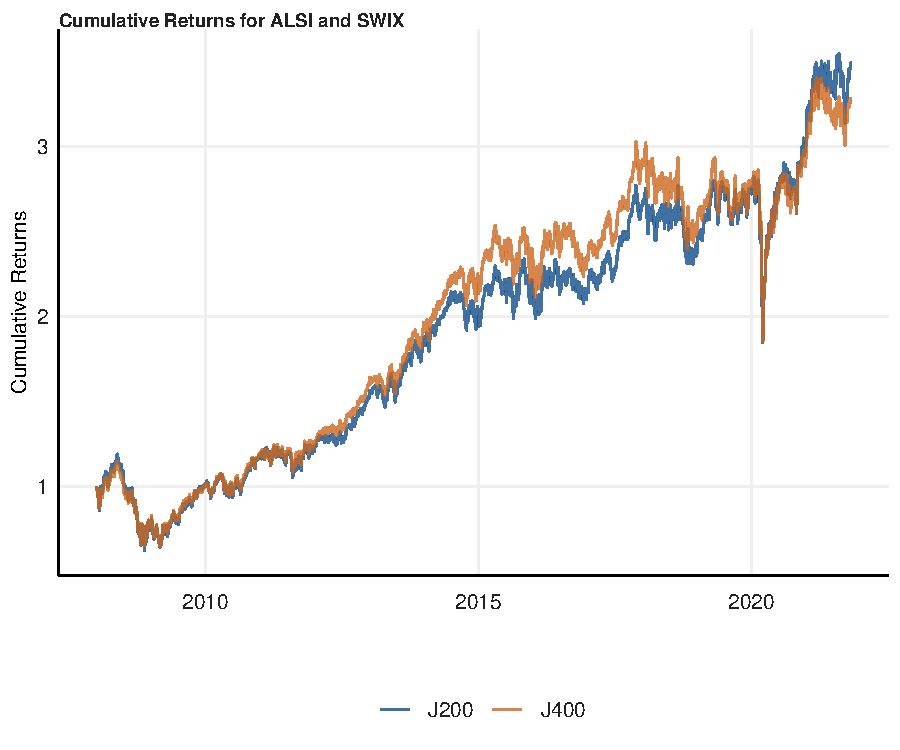
\includegraphics{Question3_files/figure-latex/unnamed-chunk-3-1.pdf}

\hypertarget{weights-plot}{%
\subsection{Weights plot}\label{weights-plot}}

An interesting look into the portfolios is to see which industries are
weighted highest between the SWIX and ALSI. Below is a plot of their
different factor weights through time. We can see that since 2020 the
ALSI lowered their weighting of Financial stocks and increased their
weighting of resource stocks in comparison to the SWIX.

\begin{itemize}
\tightlist
\item
  ALSI (J200)
\end{itemize}

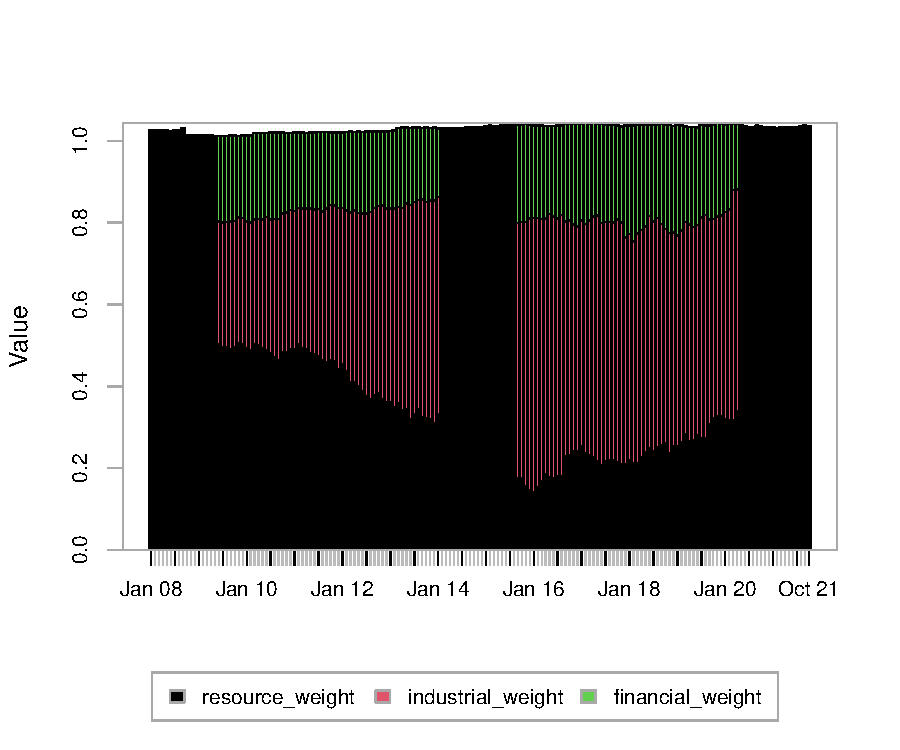
\includegraphics{Question3_files/figure-latex/unnamed-chunk-5-1.pdf}

\begin{itemize}
\tightlist
\item
  SWIX (J400)
\end{itemize}

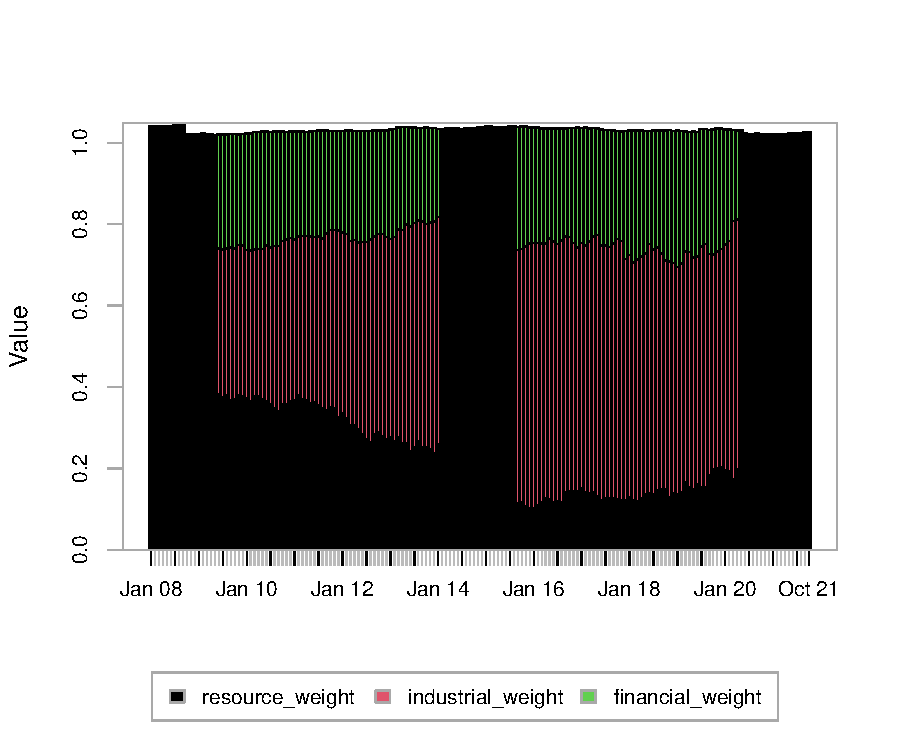
\includegraphics{Question3_files/figure-latex/unnamed-chunk-6-1.pdf}

\hypertarget{by-sector}{%
\subsection{By Sector}\label{by-sector}}

The plot below shows us the portfolio returns for the ALSI and the SWIX
across their different sectors. We can evidently see that the cumulative
returns from the Industrials is much larger that both the Financial or
Resource sectors. We can also see that the ALSI (J200) has larger
cumulative returns in both the Industrial and Resource sectors in
comparison to the SWIX (J400). However, the SWIX outperforms the ALSI in
the Financial sector.

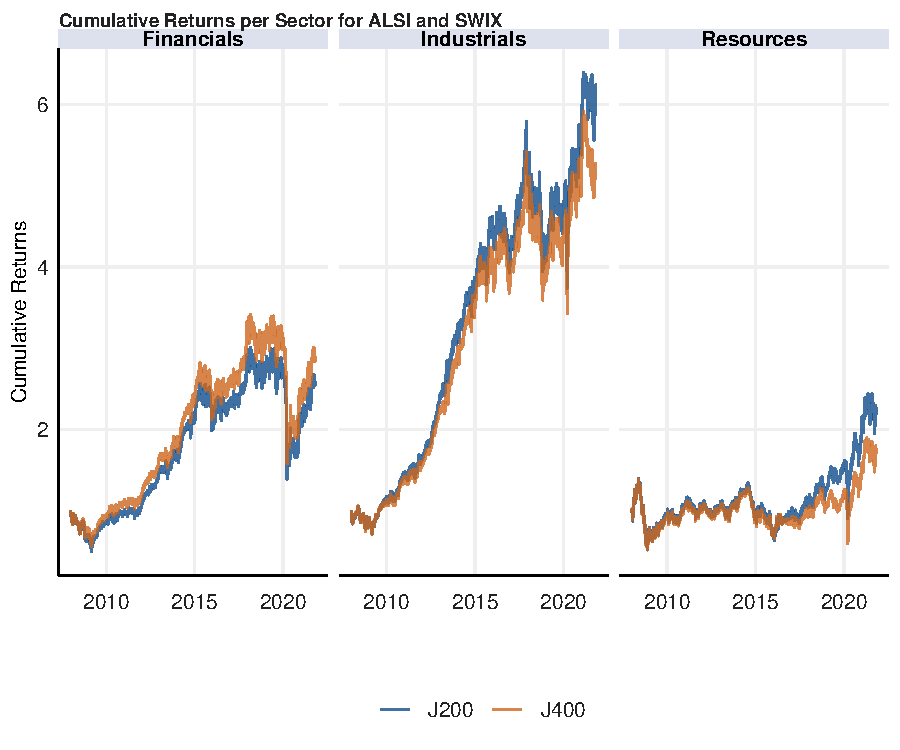
\includegraphics{Question3_files/figure-latex/unnamed-chunk-8-1.pdf}

\hypertarget{by-index-small-cap-medium-cap-and-large-cap}{%
\subsection{By Index (Small-cap, Medium-cap and
Large-cap)}\label{by-index-small-cap-medium-cap-and-large-cap}}

The plot below shows that the ALSI outperforms the SWIX for both the
Large and Mid caps. The ALSI had lower cumulative returns that the SWIX
for large caps up until 2020. There is not enough data for small caps
and thus they only contribute a very small amount of returns to either
portfolio.

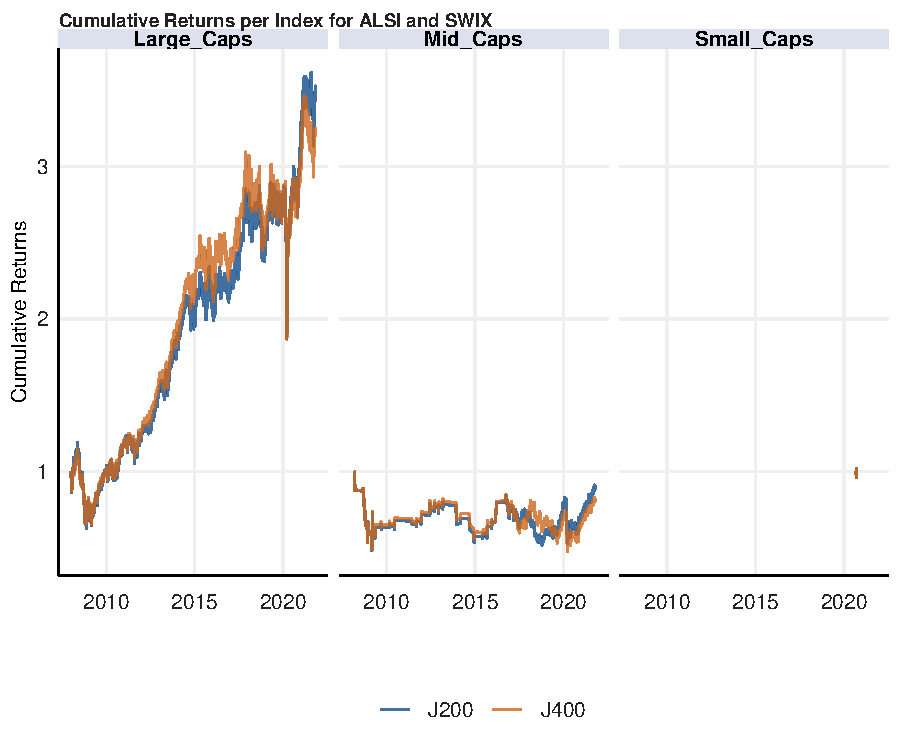
\includegraphics{Question3_files/figure-latex/unnamed-chunk-10-1.pdf}

\hypertarget{performance-during-currency-volatile-periods}{%
\section{Performance during currency volatile
periods}\label{performance-during-currency-volatile-periods}}

\hypertarget{stratify-the-returns-by-high-and-low-volatility}{%
\subsection{Stratify the returns by high and low
volatility}\label{stratify-the-returns-by-high-and-low-volatility}}

Here I find periods of high and low volatility of the USD-ZAR exchange
rate. This is done by finding a upper and lower bound of volatility to
20\%. Stratifying for these high and low volatility periods we look at
the different index's volatility (standard deviation) within those
periods.

Below is the table of volatilities during times of high exchange rate
volatility. What we can deduce is that in times of high exchange rate
volatility, the ALSI (J200) has a higher volatility than the SWIX
(J400). The SWIX also has a lower overall volatility in comparison to
the ALSI.

\begin{tabular}{l|r|r|l|r}
\hline
\multicolumn{5}{c}{High Volatility} \\
\cline{1-5}
Tickers & SD & Full\_SD & Period & Ratio\\
\hline
J200 & 0.2859593 & 0.1932903 & High\_Vol & 1.479429\\
\hline
J400 & 0.2836449 & 0.1928667 & High\_Vol & 1.470678\\
\hline
\end{tabular}

Now looking at the periods of low exchange rate volatility we can see
that the ALSI (J200) has a lower volatility than the SWIX (J400).
Although the ALSI is more volatile across the entire period when
compared to the SWIX, during periods of low volatility the ALSI is more
consistent. This can be seen with a lower ratio of volatility to full
volatility.

\begin{tabular}{l|r|r|l|r}
\hline
\multicolumn{5}{c}{Low Volatility} \\
\cline{1-5}
Tickers & SD & Full\_SD & Period & Ratio\\
\hline
J400 & 0.1537164 & 0.1928667 & Low\_Vol & 0.7970086\\
\hline
J200 & 0.1513182 & 0.1932903 & Low\_Vol & 0.7828546\\
\hline
\end{tabular}

\hypertarget{capping-of-the-indexs}{%
\section{Capping of the Index's}\label{capping-of-the-indexs}}

To evaluate the effect of capping an index we cap both the ALSI and the
SWIX at a level of 6\% and a level of 10\%, the returns based on the
differing cap levels are then graphed for both indices.

Below we can see the difference in cumulative returns of the ALSI capped
at a level of 6\% and capped at a level of 10\%. A larger cap level
clearly shows higher cumulative returns and this makes sense as if you
can have more of a high returning stock, overall returns can be higher.
Although this is also inversely true and a lower cap may force more
diversification and thus create a less risky portfolio. Cumulative
returns followed quite closely with the lower-capped index doing
marginally better until 2020 where the higher index outperformed. This
can be due to the large volatility suring this time, a higher cap can
capture more of the return.

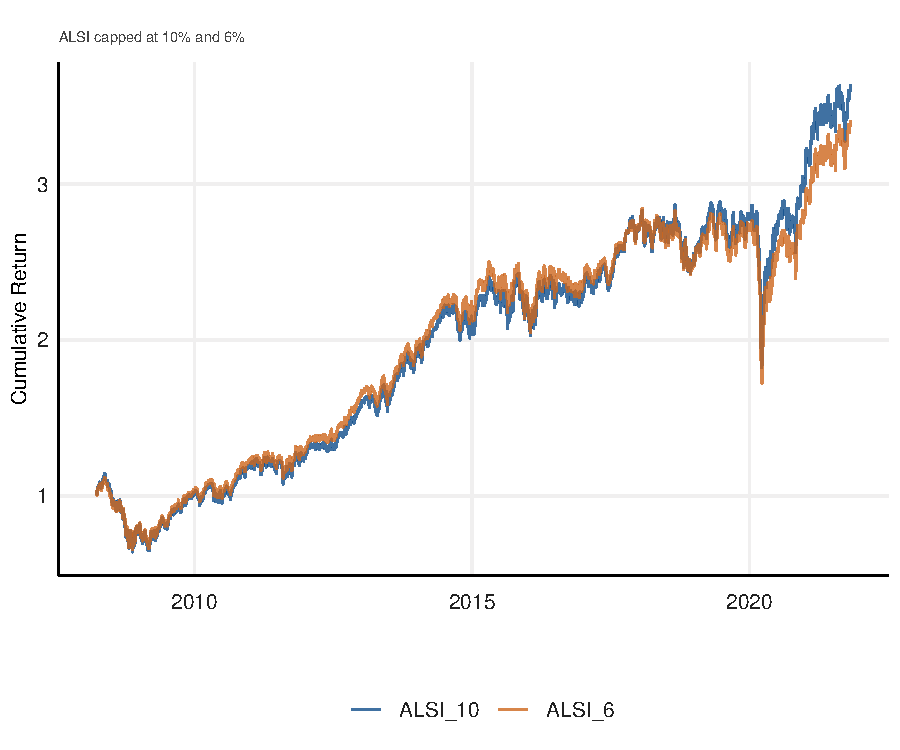
\includegraphics{Question3_files/figure-latex/unnamed-chunk-16-1.pdf}

Now for the SWIX, the results are different to that of the ALSI. The
lower-capped index actually outperformed the higher capped index.

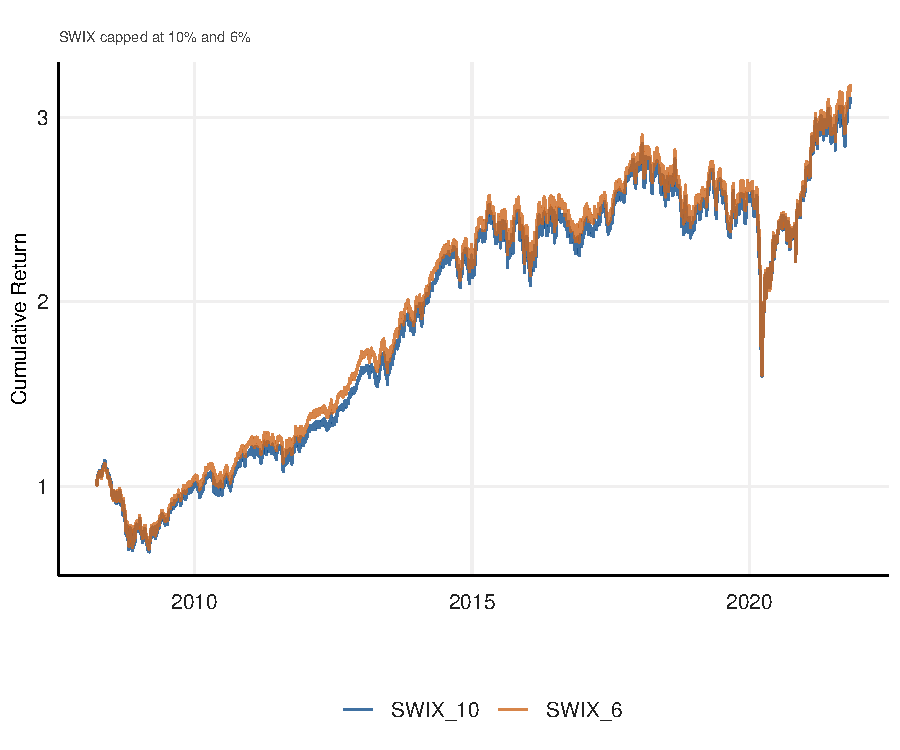
\includegraphics{Question3_files/figure-latex/unnamed-chunk-18-1.pdf}

\hypertarget{conclusion}{%
\section{Conclusion}\label{conclusion}}

What this analysis shows is that the two indexes are very similar.

\bibliography{Tex/ref}





\end{document}
